\documentclass{subfiles}

\begin{document}
	\section{Previous Work}
	
	\par Regarding the integration of FW LiDAR and hyperspectral in remote forest surveys, there are diverse opinions on whether the integration of sensors improves remote forest surveying. Clark et al attempted to estimate forest biomass but no better results were observed after the integration \cite{Clark2011}, while the outcomes of Aderson et al for observing tree species abundances structures were improved after the integration of data \cite{Anderson2008}. 
	
	\par \cite{Buddenbaum2013} Buddenbaum et al, 2013, and \cite{Heinzel2012} Heinzel and Koch, 2012, used a combination of multi-sensor data for tree classifications. Buddenbaum et al use fusion of data to generate RGB images from a combination of FW LiDAR and hyperspectral features, although the fusion reduces the dimensionality of a classifier \cite{Buddenbaum2013}. Further, in their study, three different classifiers were implemented and the Support Vector Machines (SVMs) returns the best results. SVMs were also used in \cite{Heinzel2012} to handle the high dimensionality of the metrics (464 metrics). In that research a combination of FW LiDAR, discrete LiDAR, hyperspectral and colour infrared (CIR) images are used. Each of the 125 hyperspectral bands was directly used as a feature in the classifier, contributing to the high dimensionality. 
	
	\par Here some of the FW LiDAR and LiDAR features are used but in a digested form (i.e. the width of the waveform), and matches to the spectral signatures of each class are used to reduce the dimensionality.
	
	\par To enhance the visualisation of FW LiDAR data, a volumetric approach of polygonising the data was proposed by Miltiadou et al, 2014. First, the waveforms are inserted into a 3D discrete density volume, an implicit object is defined from the volume and the object is polygonised using the Marching Cubes algorithm. In this paper we emphasis the sampling of the volume versus the sampling of the Marching Cubes algorithm as well as the effects of using full-waveform versus discrete LiDAR. Further hyperspectral imagery is introduced to improve the visual output and allow parallel interpretation of the data.
	


	
\section{Integrating hyperspectral Imagery}


	\par For every scanned area, there are both FW LiDAR and hyperspectral data, but since the data are collected from different instruments they are not aligned. To integrate the data geo-spatially, aligning the data is required. In order to preserve the highest possible quality and reduce blurring that occurs during geo-rectification, data in original sense of geometry (level 1) are used. More Information about the hyperpsectral Imagery are available in Section \ref{sec:HyperspectralImages}.
	
	\par The main idea of the geo-recification is to find the nearest hyperspectral pixel to a point in the fastest possible way. For the reason, we first import the pixels into a 2D grid, similar to \cite{Warren2014}. The dimensions of the grid and the length of squares are constant, but in our case the average number of pixels per square $(A_{ps})$ can be modified and the dimensions $(n_x, n_y)$ of the grid are calculated as follow:
	
	\begin{eqnarray}
		n_x=\sqrt{\dfrac{n_s^2}{A_{ps}}} \;\;\;\;\;\;\;\;\;\; n_y=\sqrt{\dfrac{n_l^2}{A_{ps}}}   
	\end{eqnarray} 
	
	
	
%	\begin{math}
%	 $ \sqrt[root]{2} $
	 	
%	\end{math}
	
	\par where ns = the number of samples and
	nl = the number of lines in the hyperspectral images.
	
	\par Furthermore, while Warren et al use a tree-like structure, here  structure similar to hash tables is used to speed up searching. Hash table is a data structure, which maps keys to values. In our case, we utilise the unordered\_multimap available with the standard library of the $C++$ programming language, where for every key there is a bucket with multiple values stored inside. Each square $(x_s,y_s)$	has a unique key, which is equal to $(x_s + y_s *nXs)$ and each pixel is associated with the square it lies inside. In other words, every key with its bucket corresponds to a single square of the grid and every bucket includes all the pixels that lie inside that square. The next step is for every vertex $(x_v, y_v, z_v)$ to find the pixel whose geolocation is closest it. First we project each vertex into 2D by dropping the $z$ coordinate and then we find the square $(x_s , y_s )$ that its projection $(x_v , y_v)$ lies in, as follow:
	
	**** EQUATION *****
	
	**** EQUATION *****
	\par where maxX, minX, maxY, minY = the geolocation boundaries of all the hyperspectral image.
	
	\par From the square (xs,ys) we can get the set of pixels that lie inside the same square with the vertex of our interest. Let’s assume that the positions and geolocations of these pixels are defined by $p_1	, p_2 , p_3, ... , p_n$ and $g_1, g_2, g_3 , ... , g_n$ respectively. Then, by looping through only that set of pixels, we can find the pixel $i$ that lies closest to the point $v(x_v , y_v)$
	
	**** EQUATION *****
	

	
	
		
\section{Visualisation}
	\par When the hyperspectral images are loaded along with the LiDAR files, then the outputs are: 	
	\begin{enumerate}
		\item the 3D geometry, which contains all the information about the vertices, edges, faces, normal and texture coordinates, and
		\item  a texture, which is an RGB image which is aligned with the texture coordinates of the polygon mesh.
	\end{enumerate}
	
	\par Here it worth mentioning that the texture coordinates $(u, v)$ of each vertex lies in the range $[0, 1]$ and if they are multiplied by the height/width of the texture, then the position of the corresponding pixel of the 2D texture is given. The 2D texture is simply an image generated from three user-selected bands for the RGB colours and its width is equal to the number of samples per line while its height is equal to the number of lines.
				
					
	\par DASOS projects level 1 hyperspectral images by adjusting the texture coordinates of the polygon according to the geolocation of the samples. That is, for each vertex $(xv, yv , zv)$ we find the pixel, whose geolocation $(x_g, y_g )$ is closest to it. Then by using the position of the pixel on the image $(x_p, y_p)$, the texture coordinates of the vertex are calculated accordingly.
				
	\par Finally, we need to scale the pixel position $p_i = (x_p, y_p )$, such that it lies in the range $[0,1]$. The scale factors are the number of samples $(n_s)$ and lines $(n_l)$ of the hyperspectral image. So, the texture coordinates $(u, v)$ of each vertex $v(x_v , y_v)$ are given by the following:
		
		
	**** EQUATION *****
	
	\subsection {Results}
		
		  \begin{figure} [h!]
		  	\centering
		  	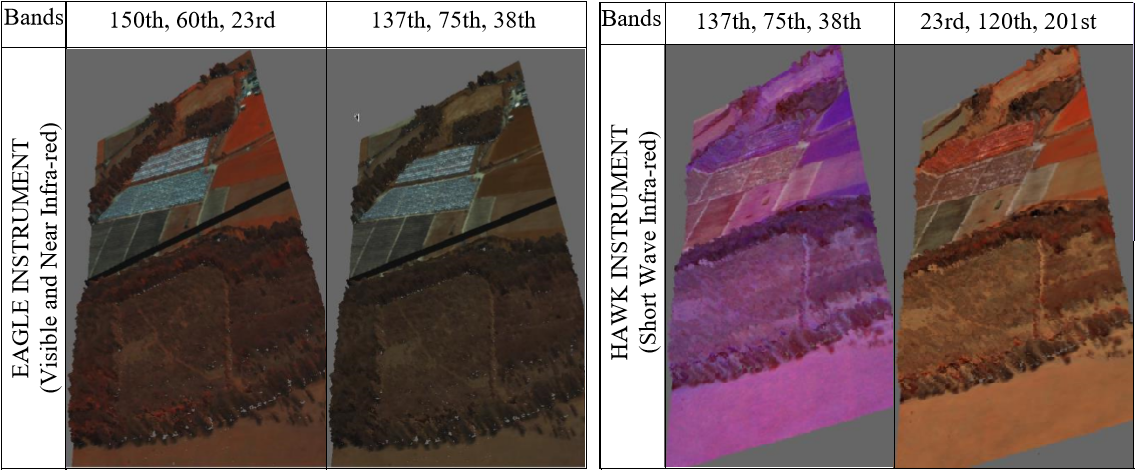
\includegraphics[width=\textwidth]{img/AlignmentEagle_Hawk}
		  	\caption[Results of Alignement]{Results of Alignment; the left table shows results of projecting hyperspectral images from the Eagle Instrument on polygonal meshes generated using FW LiDAR data and the right hand side images results using the Hawk instrument.}
		  	\label{fig:AlignementResults}
		  \end{figure}
		
		
\section{Tree Coverage Maps}

\end{document}